\section{Проектування програмного продукту}
\subsection{Концептуальне проектування}
\noindent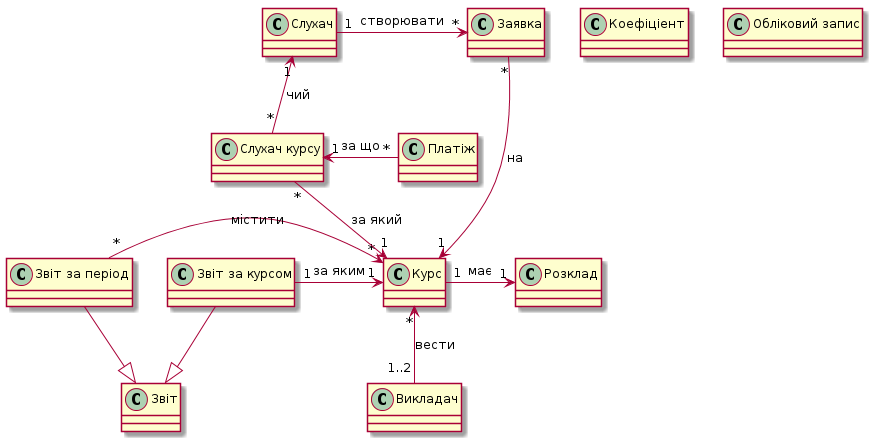
\includegraphics[width=17cm]{pp_pw3_conc.png}
\imglabel{Діаграма концептуальних класів}
\subsection{Логічне проектування}
\noindent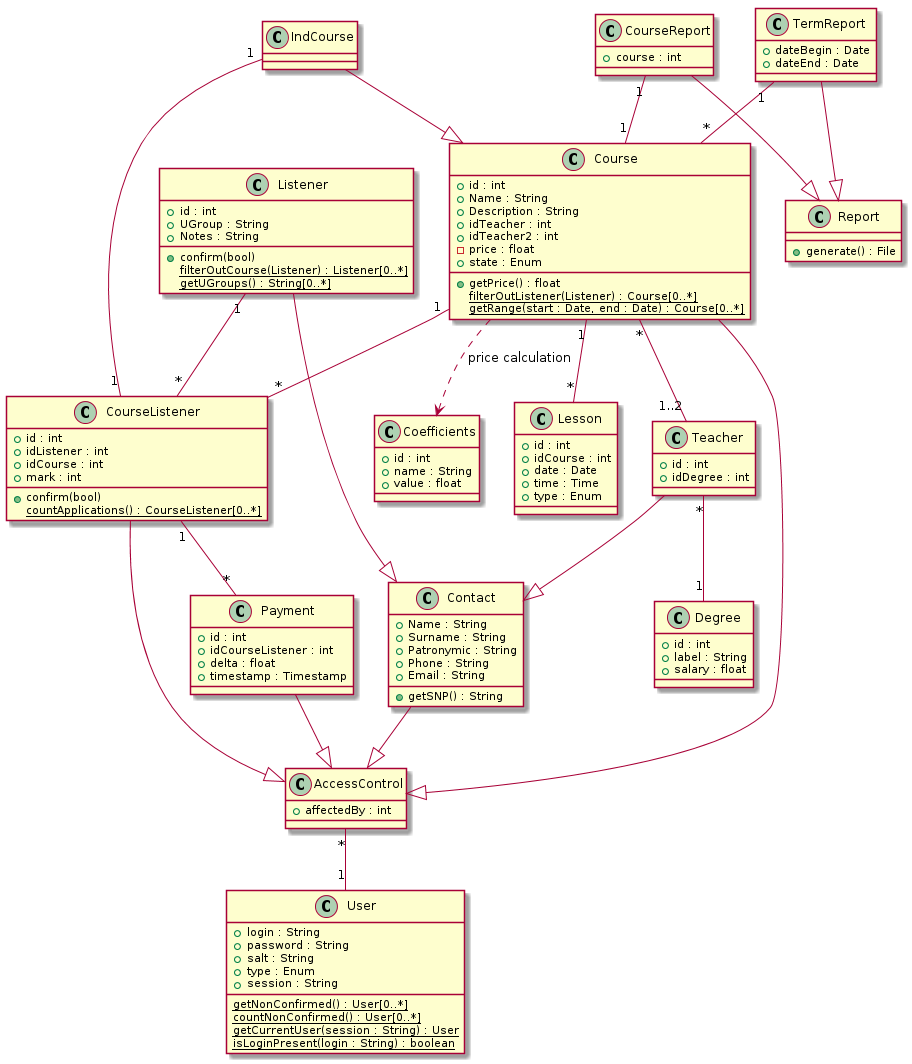
\includegraphics[width=17cm]{pp_pw3_clas.png}
\imglabel{Діаграма програмних класів}

\newpage
\subsection{База даних}
\def\dbtable#1#2#3{
 \tablabel{Опис структури таблиці "#1" (#2)}
 \begin{supertabular}{|p{1.2cm}|p{3.5cm}|p{3cm}|p{2.6cm}|p{1.2cm}|p{3.3cm}|}
 \hline
 Ключ & Назва & Ім'я поля & Тип & NULL & Дод.\\
 \hline
 #3
 \hline
 \end{supertabular}
}
\newcommand{\tabheader}[2]{
 #1 \emph{(#2)}
}
\dbtable{Слухачі}{listeners}{
PK & Ідентифікатор & idListener & int(6) & Ні & A\_I\\
 & Ім'я & Name & varchar(30) & Так & \\
 & Прізвіще & Surname & varchar(30) & Ні & \\
 & По батькові & Patronymic & varchar(30) & Так & \\
 & Університетська група & UGroup & varchar(6) & Так & \\
 & Телефон & Phone & varchar(20) & Так & \\
 & E-mail & Email & varchar(40) & Так & \\
FK & Ким змінено & affectedBy & varchar(32) & Ні & \\
}
\dbtable{Курси}{courses}{
PK & Ідентифікатор & idCourse & int(6) & Ні & A\_I\\
 & Назва & Name & varchar(50) & Ні & \\
 & Опис & Description & varchar(400) & Так & \\
 & Ознака індивідуального курсу & isIndividual & bit(1) & Ні & \\
FK & Викладач & idTeacher & int(6) & Так & \\
FK & Другий викладач & idTeacher2 & int(6) & Так & \\
 & Ціна & Price & decimal(10,2) & Так & \\
 & Кількість годин & hours & smallint(3) & Ні & \\
 & Стан & state & tinyint(1) & Ні & 0..2 (Йде набір, набрано, завершений)\\
FK & Ким змінено & affectedBy & int(6) & Ні & \\
}
\dbtable{Слухачі курсу}{Course\_Listeners}{
PK & Ідентифікатор & idCL & int(6) & Ні & A\_I\\
FK & Курс & idCourse & int(6) & Ні & \\
FK & Слухач & idListener & int(6) & Ні & \\
 & Оцінка & mark & tinyint(3) & Так & \\
FK & Ким змінено & affectedBy & int(6) & Ні & \\
}
\newpage
\dbtable{Платежі}{payments}{
PK & Ідентифікатор & idPayment & int(6) & Ні & A\_I\\
FK & Слухач курсу & idCL & int(6) & Ні & \\
 & Кошти & delta & int(6) & Ні & \\
 & Мітка часу & timestamp & timestamp & Ні & CURRENT\_\ TIMESTAMP\\
}
\dbtable{Викладачі}{teachers}{
PK & Ідентифікатор & idTeacher & int(6) & Ні & A\_I\\
 & Ім'я & Name & varchar(30) & Так & \\
 & Прізвіще & Surname & varchar(30) & Ні & \\
 & По батькові & Patronymic & varchar(30) & Так & \\
 & Телефон & Phone & varchar(20) & Так & \\
 & E-mail & Email & varchar(40) & Так & \\
FK & Ким змінено & affectedBy & varchar(32) & Ні & \\
FK & Вчений ступінь & degree & tinyint(2) & Так & \\
}
\dbtable{Розцінки}{prices}{
PK & Ідентифікатор & degree & tinyint(2) & Ні & A\_I\\
 & Вчений ступінь & deglab & varchar(30) & Ні & \\
 & Зарплата & salary & decimal(10,2) & Ні & \\
}
\dbtable{Коефіціенти}{coefficients}{
PK & Ідентифікатор & idCoefficient & tinyint(2) & Ні & A\_I\\
 & Мітка & name & varchar(128) & Так & \\
 & Значення & value & float & Так & \\
}
\dbtable{Заняття}{lessons}{
PK & Ідентифікатор & idLesson & int(11) & Ні & A\_I\\
FK & Курс & idCourse & int(11) & Ні & \\
 & Дата & date & date & Так & \\
 & Час початку & time & time & Ні & \\
 & Тип & type & tinyint(1) & Ні & 0..1 (Лекція, Практика)\\
}
\newpage
\dbtable{Користувачі}{users}{
PK & Логін & login & varchar(32) & Ні & \\
 & Хеш паролю & password & text & Ні & \\
 & Сіль & salt & text & Ні & \\
 & Тип & isAdmin & tinyint(1) & Ні & 0..2 (Оператор, Адміністратор, Переглядач)\\
 & Ключ сесії & sessionid & text & Так & \\
}

\subsection{Оцінка алгоритмічної складності}

\tikzset{
	line/.style={draw, -latex'},
	every join/.style={line},
	u/.style={anchor=south},
	r/.style={anchor=west},
	fxd/.style={text width = 6em},
	it/.style={font={\small\itshape}},
	bf/.style={font={\small\bfseries}}
}
\tikzstyle{base} =
	[
		draw,
		on chain,
		on grid,
		align=center,
		minimum height=4ex,
		minimum width = 10ex,
		node distance = 6mm and 60mm,
		text badly centered
	]
\tikzstyle{coord} =
	[
		coordinate,
		on chain,
		on grid
	]
\tikzstyle{cloud} =
	[
		base,
		ellipse,
		fill = red!5,
		node distance = 3cm,
		minimum height = 2em
	]
\tikzstyle{decision} =
	[
		base,
		diamond,
		aspect=2,
		fill = green!10,
		node distance = 2cm,
		inner sep = 0pt
	]
\tikzstyle{block} =
	[
		rectangle,
		base,
		fill = blue!3,
		rounded corners,
		minimum height = 2em
	]
\tikzstyle{print_block} =
	[
		base,
		tape,
		tape bend top=none,
		fill = yellow!10
	]
\tikzstyle{io} =
	[
		base,
		trapezium,
		trapezium left angle = 70,
		trapezium right angle = 110,
		fill = blue!5
	]
\makeatletter
\pgfkeys{/pgf/.cd,
	subrtshape w/.initial=2mm,
	cycleshape w/.initial=2mm
}
\pgfdeclareshape{subrtshape}{
	\inheritsavedanchors[from=rectangle]
	\inheritanchorborder[from=rectangle]
	\inheritanchor[from=rectangle]{north}
	\inheritanchor[from=rectangle]{center}
	\inheritanchor[from=rectangle]{west}
	\inheritanchor[from=rectangle]{east}
	\inheritanchor[from=rectangle]{mid}
	\inheritanchor[from=rectangle]{base}
	\inheritanchor[from=rectangle]{south}
	\backgroundpath{
		\southwest \pgf@xa=\pgf@x \pgf@ya=\pgf@y
		\northeast \pgf@xb=\pgf@x \pgf@yb=\pgf@y
		\pgfmathsetlength\pgfutil@tempdima{\pgfkeysvalueof{/pgf/subrtshape w}}
		\def\ppd@offset{\pgfpoint{\pgfutil@tempdima}{0ex}}
		\def\ppd@offsetm{\pgfpoint{-\pgfutil@tempdima}{0ex}}
		\pgfpathmoveto{\pgfqpoint{\pgf@xa}{\pgf@ya}}
		\pgfpathlineto{\pgfqpoint{\pgf@xb}{\pgf@ya}}
		\pgfpathlineto{\pgfqpoint{\pgf@xb}{\pgf@yb}}
		\pgfpathlineto{\pgfqpoint{\pgf@xa}{\pgf@yb}}
		\pgfpathclose
		\pgfpathmoveto{\pgfpointadd{\pgfpoint{\pgf@xa}{\pgf@yb}}{\ppd@offsetm}}
		\pgfpathlineto{\pgfpointadd{\pgfpoint{\pgf@xa}{\pgf@ya}}{\ppd@offsetm}}
		\pgfpathlineto{\pgfpointadd{\pgfpoint{\pgf@xb}{\pgf@ya}}{\ppd@offset}}
		\pgfpathlineto{\pgfpointadd{\pgfpoint{\pgf@xb}{\pgf@yb}}{\ppd@offset}}
		\pgfpathclose
	}
}
\pgfdeclareshape{cyclebegshape}{
	\inheritsavedanchors[from=rectangle]
	\inheritanchorborder[from=rectangle]
	\inheritanchor[from=rectangle]{north}
	\inheritanchor[from=rectangle]{center}
	\inheritanchor[from=rectangle]{west}
	\inheritanchor[from=rectangle]{east}
	\inheritanchor[from=rectangle]{mid}
	\inheritanchor[from=rectangle]{base}
	\inheritanchor[from=rectangle]{south}
	\backgroundpath{
		\southwest \pgf@xa=\pgf@x \pgf@ya=\pgf@y
		\northeast \pgf@xb=\pgf@x \pgf@yb=\pgf@y
		\pgfmathsetlength\pgfutil@tempdima{\pgfkeysvalueof{/pgf/cycleshape w}}
		\pgfpathmoveto{\pgfqpoint{\pgf@xa}{\pgf@ya}}
\pgfpathlineto{\pgfpointadd{\pgfpoint{\pgf@xa}{\pgf@yb}}{\pgfpoint{0ex}{-\pgfutil@tempdima}}}
\pgfpathlineto{\pgfpointadd{\pgfpoint{\pgf@xa}{\pgf@yb}}{\pgfpoint{\pgfutil@tempdima}{0ex}}}
\pgfpathlineto{\pgfpointadd{\pgfpoint{\pgf@xb}{\pgf@yb}}{\pgfpoint{-\pgfutil@tempdima}{0ex}}}
\pgfpathlineto{\pgfpointadd{\pgfpoint{\pgf@xb}{\pgf@yb}}{\pgfpoint{0ex}{-\pgfutil@tempdima}}}
\pgfpathlineto{\pgfqpoint{\pgf@xb}{\pgf@ya}}
		\pgfpathclose
	}
}
\pgfdeclareshape{cycleendshape}{
	\inheritsavedanchors[from=rectangle]
	\inheritanchorborder[from=rectangle]
	\inheritanchor[from=rectangle]{north}
	\inheritanchor[from=rectangle]{center}
	\inheritanchor[from=rectangle]{west}
	\inheritanchor[from=rectangle]{east}
	\inheritanchor[from=rectangle]{mid}
	\inheritanchor[from=rectangle]{base}
	\inheritanchor[from=rectangle]{south}
	\backgroundpath{
		\southwest \pgf@xa=\pgf@x \pgf@ya=\pgf@y
		\northeast \pgf@xb=\pgf@x \pgf@yb=\pgf@y
		\pgfmathsetlength\pgfutil@tempdima{\pgfkeysvalueof{/pgf/cycleshape w}}
		\pgfpathmoveto{\pgfqpoint{\pgf@xb}{\pgf@yb}}
\pgfpathlineto{\pgfpointadd{\pgfpoint{\pgf@xb}{\pgf@ya}}{\pgfpoint{0ex}{\pgfutil@tempdima}}}
\pgfpathlineto{\pgfpointadd{\pgfpoint{\pgf@xb}{\pgf@ya}}{\pgfpoint{-\pgfutil@tempdima}{0ex}}}
\pgfpathlineto{\pgfpointadd{\pgfpoint{\pgf@xa}{\pgf@ya}}{\pgfpoint{\pgfutil@tempdima}{0ex}}}
\pgfpathlineto{\pgfpointadd{\pgfpoint{\pgf@xa}{\pgf@ya}}{\pgfpoint{0ex}{\pgfutil@tempdima}}}
\pgfpathlineto{\pgfqpoint{\pgf@xa}{\pgf@yb}}
		\pgfpathclose
	}
}
\makeatother
\tikzstyle{subroutine} =
	[
		base,
		subrtshape,
		fill = green!25
	]
\tikzstyle{cyclebegin} =
	[
		base,
		cyclebegshape,
		fill = blue!25
	]
\tikzstyle{cycleend} =
	[
		base,
		cycleendshape,
		fill = blue!25
	]
\tikzstyle{connector} =
	[
		base,
		circle,
		fill = red!25,
		minimum width = 3mm
	]

\begin{center}
{ \fontsize{10pt}{12pt} \selectfont
\begin{tikzpicture}[%
    start chain=going below,
    node distance=5mm and 60mm,
        ]
        \node [cloud] (start) {getCoursePrice(id, full, verif)};
	\node [block, join] (global) {PRICE\_TRUNK := 10};
	\node [decision, join] (argcond1) {verif = false};
	\node [block] (setarg1) {verif := true};
	\node [connector, join] (join1) {};
	\node [block, join] (q1) {price := вартість з таблиці courses\\для курсу id,\\ hours := кількість годин з таблиці courses\\для курсу id};
	\node [decision, join] (q1cond) {price = 0};
	\node [block, join] (q2) {count := кількість слухачів\\з таблиці Course\_Listeners\\для курсу id};
	\node [block, join] (q3) {salary := (зарплата з таблиці prices\\для вченого ступеню з таблиці teachers\\для викладача з таблиці courses) *\\(кількість занять з таблиці lessons\\з типом <<Лекція>>) + (зарплата з таблиці prices\\для вченого ступеню з таблиці teachers\\для другого викладача з таблиці courses) *\\(кількість занять з таблиці lessons\\з типом <<Практика>>)};
        \node [subroutine, join, subrtshape w = 3mm, fxd] (coefficients) {coef := getCoefficients()};
	\node [block, join] (price) {price := $\left[ \frac{salary \cdot coef.personal \cdot coef.bonus \cdot coef.others \cdot hours}{count \cdot PRICE\_TRUNK}\right] \cdot PRICE\_TRUNK$};
	\node [decision, join] (fullcond) {full};
	\node [block] (fullmul) {price := $price \cdot count$};
        \node [cloud, join] (finish) {Повернення price};

        \path [line] (argcond1) to node [r] {Так} (setarg1);
        \path [line] (argcond1) -- node [u,near start] {Ні} ++(5cm, 0cm) |- (join1);
        \path [line] (q1cond) to node [r] {Так} (q2);
        \path [line] (q1cond) -- node [u,near start] {Ні} ++(7cm, 0cm) |- (finish);
        \path [line] (fullcond) to node [r] {Так} (fullmul);
        \path [line] (fullcond) -- node [u,near start] {Ні} ++(3cm, 0cm) |- (finish);
\end{tikzpicture}
}
\end{center}
\imglabel{Алгоритм розрахунку вартості курсу}

\begin{center}
{ \fontsize{10pt}{12pt} \selectfont
\begin{tikzpicture}[%
    start chain=going below,
    node distance=5mm and 60mm,
        ]
        \node [cloud] (start) {user\_login(login, pass)};
	\node [block, join] (config) {config := з файлу конфігурації};
	\node [block, join] (q1) {user[password, salt, sessionid] := з\\таблиці users для логіну login};
	\node [decision, join] (q1cond) {user = $\emptyset$};
	\node [decision, yshift=-3mm] (confcond) {sessionid = <<q>>};
	\node [block] (crypt) {hash := crypt(pass,\\config.global\_salt)};
	\node [decision, join] (passcond) {pass = hash};
	\node [block] (gensess) {sess\_id := randhash(login, 500)};
	\node [block, join] (updsess) {Встановити в\\таблиці users\\sessionid := sess\_id\\для логіну login};
	\node [block, join] (cookiesess) {Записати sess\_id в Cookies};
	\node [block, join] (gotomain) {Перейти на головну сторінку};
        \node [cloud, join] (finish) {Вихід};

	\node [block, right of = q1cond, node distance = 8cm, yshift = -5mm] (err5) {Помилка 400:\\користувача не знайдено};
	\node [block, right of = confcond, node distance = 6.2cm, yshift = -5mm] (err10) {Помилка 403:\\обліковий запис\\ще не підтверджено};
	\node [block, right of = passcond, node distance = 4.5cm, yshift = -5mm] (err6) {Помилка 403:\\пароль невірний};

        \path [line] (q1cond) to node [r] {Ні} (confcond);
        \path [line] (q1cond) -| node [u,near start] {Так} (err5);
        \path [line] (err5) |- node {} (finish);
        \path [line] (confcond) to node [r] {Ні} (crypt);
        \path [line] (confcond) -| node [u,near start] {Так} (err10);
        \path [line] (err10) |- node {} (finish);
        \path [line] (passcond) to node [r] {Так} (gensess);
        \path [line] (passcond) -| node [u,near start] {Ні} (err6);
        \path [line] (err6) |- node {} (finish);
\end{tikzpicture}
}
\end{center}
\imglabel{Алгоритм аутентифікації та авторизації}

На рис. 3 зазначено складну операцію розрахунку вартості за даними з БД. Вона реалізується наступним SQL-запитом:
{ \fontsize{10pt}{12pt} \selectfont
\begin{verbatim}
SELECT ifnull(s1,0)*ifnull(c1,0)+ifnull(s2,0)*ifnull(c2,0) FROM ((
 SELECT salary as s1 FROM prices WHERE degree IN (
  SELECT degree FROM teachers WHERE idTeacher IN (
   SELECT idTeacher FROM courses WHERE idCourse=?
))) s1 LEFT OUTER JOIN (
 SELECT salary as s2 FROM prices WHERE degree IN(
  SELECT degree FROM teachers WHERE idTeacher IN (
   SELECT idTeacher2 FROM courses WHERE idCourse=63
))) s2 ON 1=1) LEFT OUTER JOIN ((
 SELECT count(*) as c1 FROM lessons WHERE idCourse=? AND type=0
) c1 ON 1=1 LEFT OUTER JOIN (
 SELECT count(*) as c2 FROM lessons WHERE idCourse=? AND type=1
) c2) ON 1=1;
\end{verbatim}
}

План виконання запиту:
\begin{enumerate}
\setlength{\itemsep}{0pt}
\item Вибірка вмісту таблиці courses
\item Проекція кортежів за значенням атрибуту idCourse
\item Проекція атрибутів за атрибутом idCourse
\item Вибірка вмісту таблиці teachers
\item Проекція кортежів за значенням атрибуту idTeacher
\item Проекція атрибутів за атрибутом degree
\item Вибірка вмісту таблиці prices
\item Проекція кортежів за значенням атрибуту degree
\item Проекція атрибутів за атрибутом salary
\item Використання вибірки з п. 1.
\item Проекція кортежів за значенням атрибуту idCourse
\item Проекція атрибутів за атрибутом idCourse
\item Використання вибірки з п. 4.
\item Проекція кортежів за значенням атрибуту idTeacher
\item Проекція атрибутів за атрибутом degree
\item Використання вибірки з п. 7.
\item Проекція кортежів за значенням атрибуту degree
\item Проекція атрибутів за атрибутом salary
\item Вибірка вмісту таблиці lessons
\item Проекція кортежів за значенням атрибуту idCourse
\item Проекція кортежів за значенням атрибуту type
\item Підрахунок кортежів
\item Використання проекції з п. 20.
\item Проекція кортежів за значенням атрибуту type
\item Підрахунок кортежів
\item З'єднання результатів пп. 9 та 18.
\item З'єднання результатів пп. 22 та 25.
\item З'єднання результатів пп. 26 та 27.
\item Розрахунок математичного виразу за результатом п. 28.
\end{enumerate}

Операції проекції кортежів у пп. 2, 3, 5, 6, 8, 9, 11, 12, 14, 15, 17 та 18 повинні повертати один кортеж. Пошук у таблицях courses та teachers відбувається за первинним ключем, а таблиця prices складається з кількох кортежів. Для проекцій з пп. 20, 21 та 24 доцільно створити у таблиці lessons індекс за атрибутом idCourse. За атрибутом type індекс недоцільний, оскільки проекції за ним відбуваються не з усієї таблиці, а можливих значення тільки два. SQL-запит для створення індексу:
\begin{verbatim}
CREATE INDEX course_of_lesson ON lessons (idCourse);
\end{verbatim}

Циклів в алгоритмах на рис. 3 та 4 немає, тож їх складність --- O(N).

\subsection{Опис зовнішних інтерфейсів}

Інтерфейс користувача побудовано із використанням бібліотеки Kendo UI, дизайн визначається наявними для неі темами оформлення. Доступні самостійні концептуальні класи присутні у головному меню та розташовані за частотою використання: найактивніша робота проводиться зі слухачами та курсами, викладачі та користувачі заповнюються на початку роботи і потім змінюються рідко, звіти здаються рідко, розцінки та коефіціенти змінюються у виключних випадках. В кінці головного меню розміщено кнопку виходу з системи. Екрану авторизації є окремим та лаконічним, містить лише форму та кнопку перемикання форм реєстрації та входу.

Для роботи серверної частини системи потрібен веб-сервер Apache 2.x, інтерпретатор PHP5 не нижче 5.4, СКБД MySQL або MariaDB 5. Для користування клієнтською частиною потрібен web-браузер із підтримкою EcmaScript 5; тестування проводиться у поточних версіях браузерів Mozilla Firefox та Chromium для десктопу.

Система може працювати у межах однієї машини, через локальну мережу та через мережу Інтернет, в залежності від мережевих підключень та налаштувань машини, на якій встановлено серверну частину. Підключення, відповідно, може здійснюватись будь-яким доступним дротовим або бездротовим каналом підключення до локальної мережі або мережі Інтернет: Ethernet, Wi-Fi, ADSL, HSPA, Dial-up та ін. Оскільки звіти генеруються у форматі PDF, для їх перегляду потрібна програма --- переглядач PDF: Mozilla Firefox, Google Chrome, Adobe Reader, Foxit Reader тощо. Для друку потрібен принтер, підключений безпосередньо до машини, на якій відкрито файл звіту, або доступний для неї через мережу.
